\chapter{Solución Propuesta}
Se plantea desarrollar una aplicación web que permita a empresas la aplicación de encuestas, pruebas, cuestionarios, test y/o instrumentos de medición de percepción u opiniones sobre aspectos relevantes para la organización. La solución a desarrollar está basada en la siguiente arquitectura:



Adicionalmente, se propone el uso de un API de un encuestador. El cual interactuará de la siguiente forma con la aplicación a desarrollar

% \begin{figure}[t]
% \centering
% 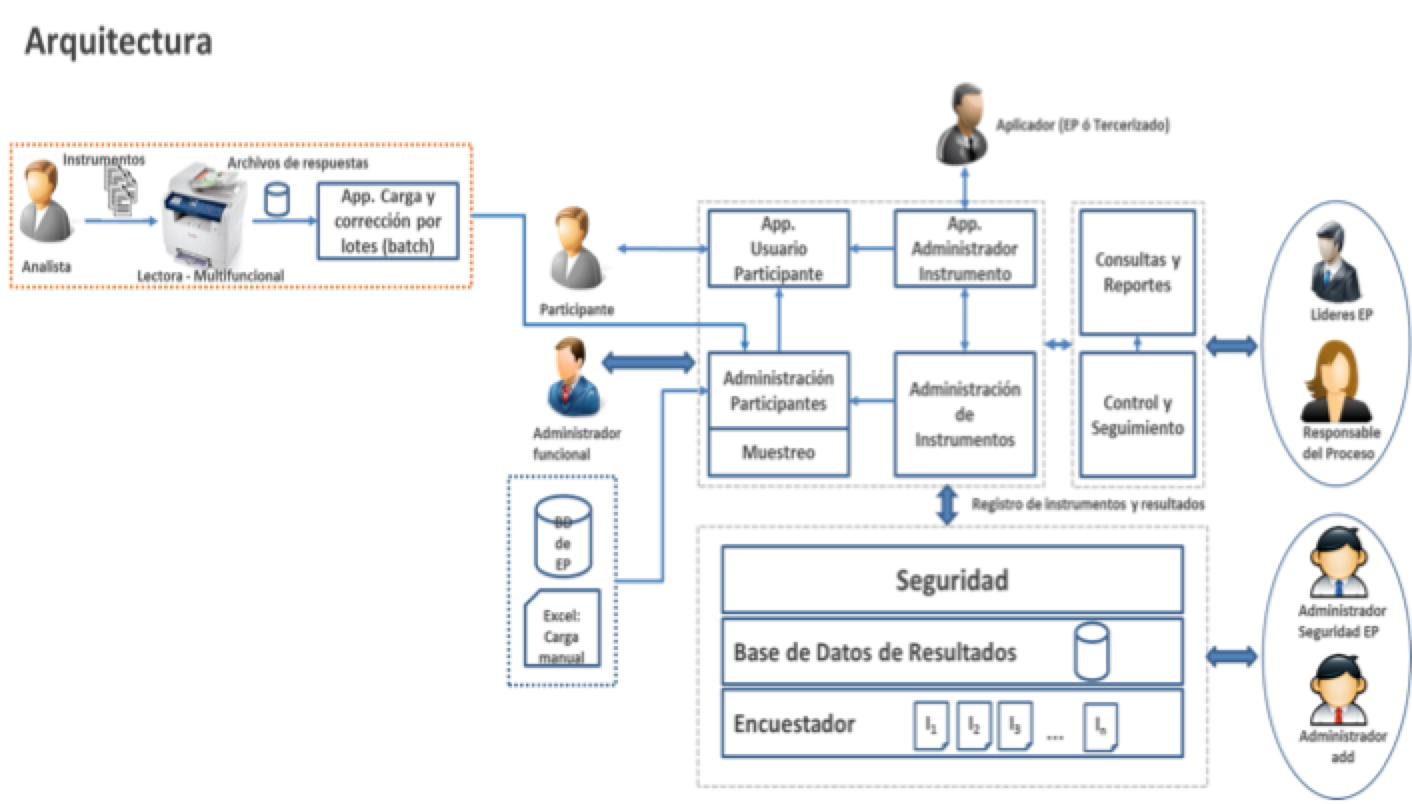
\includegraphics[scale=0.5]{imagenes/arquitectura}
% \caption{Arquitectura del sistema}
% \label{fig:arquitectura}
% 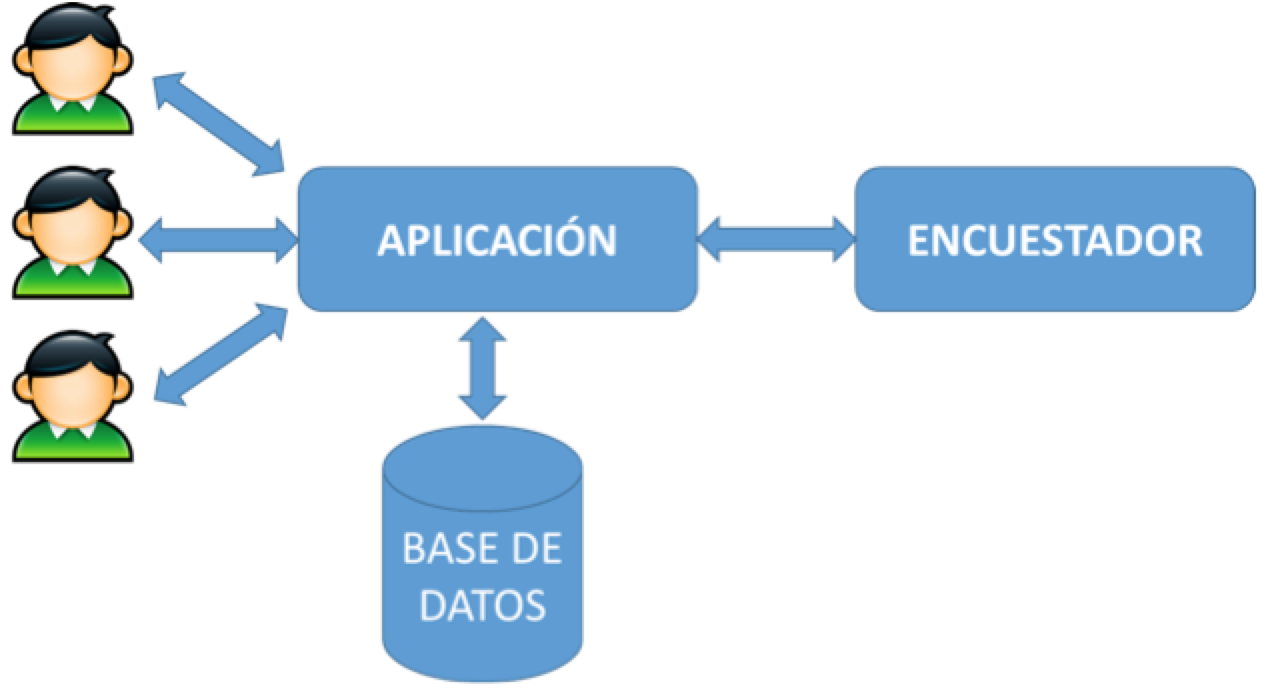
\includegraphics[scale=0.5]{imagenes/arquitectura_resumida}
% \caption{Diagrama del sistema}
% \label{fig:arquitectura_resumida}
% 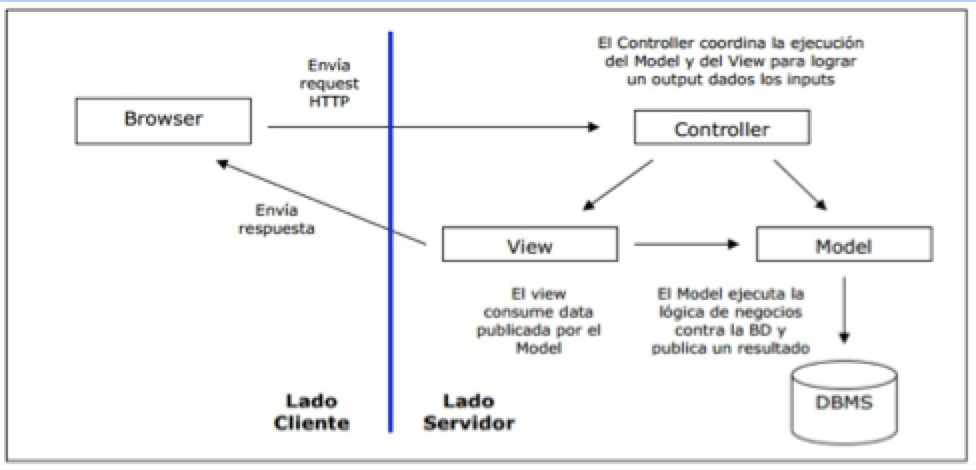
\includegraphics[scale=0.5]{imagenes/mvc_dinamica}
% \caption{Arquitectura MVC del framework Dinámica}
% \label{fig:mvc_dinamica}
% \end{figure}

El software será desarrollado bajo el patrón de arquitectura Modelo Vista Controlador (MVC), el cual es un modelo que se basa en tres capas: Modelo, Vista y Controlador. Cada capa maneja información diferente, lo cual es beneficioso para cualquier software ya que se separan los conceptos y se tiene un trabajo más ordenado.

